% Independent two-column proof. Compile with latexmk -pdf arbitration-proof.tex.
\documentclass[sigconf,nonacm]{acmart}
\usepackage{stfloats}
\setcopyright{none}
\settopmatter{printacmref=false,printfolios=true}
\title{Safety and Liveness of an Arbitration Protocol Model}
% A standalone report has no proceedings publisher in its PDF metadata.
\makeatletter
\let\hyxmp@parse@acmart\relax
\makeatother
\hypersetup{pdftitle={Safety and Liveness of an Arbitration Protocol Model},
  pdfsubject={Safety and conditional liveness for an arbitration protocol model},hidelinks}

\newcommand{\acc}{\mathit{acc}}
\newcommand{\lsn}{\mathrm{LSN}}

\begin{document}
\maketitle
\hypersetup{pdfcreator={LaTeX},pdfsubject={Safety and conditional liveness for an arbitration protocol model}}
\pagestyle{plain}
\thispagestyle{plain}
\raggedbottom
\appendix
\section{Safety and Liveness Proofs}

Full replicas \(F_1, F_2, \ldots\) store redo for a replicated log stream;
the arbitration replica \(A\) stores only protocol metadata and votes in
elections and membership changes. A log sequence number (LSN) indexes
entries. For the protocol model below, Theorem~4.3 shows that, upon
completing log recovery, a full-replica leader holds every entry
committed in a lower-numbered proposal, even across membership changes;
Theorem~4.4 gives sufficient conditions to resume committing writes.
Theorem numbering follows \emph{Arbitration Without Redo: Data-less
Voting for Site-Level Disaster Recovery in OceanBase} by Quanqing Xu,
Chen Qian, and colleagues~\cite{arbitration}; Figure~\ref{fig:confirmation}
reproduces its Figure~4.

\noindent\textsc{Theorem 4.3 (Safety).}
\emph{Suppose entry \(e\) is committed at LSN \(i\) under proposal
number \(p\).}
\begin{enumerate}
  \item[\emph{(a)}] \emph{Leader completeness. Every full-replica leader
    of a proposal \(q>p\) holds \(e\) at \(i\) upon completing log recovery.}
  \item[\emph{(b)}] \emph{Agreement. No other entry can be committed at \(i\).}
\end{enumerate}

\par\addvspace{\medskipamount}
\noindent\fbox{\begin{minipage}{\dimexpr\columnwidth-2\fboxsep-2\fboxrule\relax}
\small\setlength{\parskip}{2pt}\setlength{\parindent}{0pt}
\textbf{Protocol summary.} One log stream; the premises below state each rule
in full.

\textbf{State.} Every voter durably stores \(\mathit{promise}\) and its
installed configuration \(\mathit{config}\); a full replica also stores its
redo \(\mathrm{log}\) and accepted ballot \(\acc\). The arbiter \(A\) stores
no redo. \(P_C=S_C\cup\{A\}\).

\textbf{Quorums.} Prepare quorum: majority of \(P_C\). Accept quorum:
majority of \(S_C\). A configuration is confirmed by a majority of its own
election membership.

\textbf{R1 Prepare\((q,V)\).} Grant iff \(q>\mathit{promise}\) and
\(V\ge\mathit{config}\); durably set \(\mathit{promise}:=q\); a full replica
replies with \((\acc,\mathrm{log})\).

\textbf{R2 Recovery.} Adopt the longest log with the highest \(\acc\) among
full-replica replies in the prepare quorum; then propose only extensions of
it, append-only.

\textbf{R3 Accept\((t,P)\).} Grant iff \(t\ge\mathit{promise}\); Accept is
the only transition that updates \((\acc,\mathrm{log})\).

\textbf{R4 Confirmation.} After recovery in \(t\), confirm the inherited
membership with a majority of its election voters before proposing any
prefix or membership change. A voter confirms \(W\) in \(t\) iff
\(t\ge\mathit{promise}\) and \(W\ge\mathit{config}\).

\textbf{R5 Single-member change.} Add or remove one full replica. Before
publishing \(M\), an accept quorum of \(S_M\) accepts the current prefix in
\(t\); use \(M\)'s accept quorum, or publish another change, only after a
majority of \(P_M\) confirms \(M\) in \(t\).

\textbf{R6 Commit freeze.} From selecting the pre-change prefix until \(M\)
is confirmed, the old configuration's commit point does not advance, and the
change is never canceled to resume committing under the old configuration.

\textbf{R7 Commit.} An entry commits in \(p\) once an accept quorum of the
effective configuration's \(S\) has accepted the prefix through it in \(p\).

\textbf{R8 Arbiter.} \(A\) issues no configurations and no redo; as election
leader it only forwards its installed configuration, which receivers adopt
without changing \(\mathit{promise}\), \(\acc\), or \(\mathrm{log}\).

\emph{Dependencies.} Theorem~4.3 relies only on R1--R8 and the failure model;
Theorem~4.4 additionally uses the progress assumptions of
Section~\ref{sec:liveness}. Failure detection and degradation policy decide
which replica is degraded and when; they affect liveness and redundancy, not
safety.
\end{minipage}}
\par\addvspace{\medskipamount}

\subsection*{Protocol premises}
\begingroup
\setlength{\parindent}{0pt}
\setlength{\parskip}{0.25\baselineskip}
\textbf{Failure model.} We consider one log stream with non-Byzantine
replicas that may crash and restart with durable state intact. Messages
may be delayed, lost, duplicated, or reordered, and the network may
partition (progress conditions appear in Section~\ref{sec:liveness}).

\textbf{Configurations and quorums.} In configuration \(C\), let \(S_C\)
be the nonempty set of full replicas in the log commit membership and let
\(P_C=S_C\cup\{A\}\) be the election membership. An \emph{accept quorum}
is a majority of \(S_C\), and a \emph{prepare quorum} is a majority of
\(P_C\). Only full replicas store and supply redo. Each voter durably
stores its locally installed configuration (initially \(C_0\)), separate
from the redo log, and updates it only in nondecreasing version order
(ordered by issuing proposal number, then publication order).

\textbf{Prepare, recovery, and Accept.} Each voter durably records its
highest promised or voted proposal number \(\mathit{promise}\)
(initially \(0\)) and executes \(\mathrm{Prepare}\), \(\mathrm{Accept}\),
and confirmation check-and-updates atomically. Following Generalized
Paxos~\cite[\S5.3]{lamport}, each full replica also durably records its
log prefix \(\mathrm{log}\) (initially empty, end LSN \(\ell=0\)) and
accepted ballot \(\acc\) (initially \(0\)), the highest proposal number
in which it accepted its current prefix.
\emph{Prepare:} A candidate chooses a proposal number \(q\) above every
proposal number it has observed (exceeding its \(\mathit{promise}\) and
installed configuration's proposal) and fixes its installed
configuration \(V\). A voter grants \(\mathrm{Prepare}(q,V)\) only if
\(q>\mathit{promise}\) and \(V\ge\mathit{config}\), durably setting
\(\mathit{promise}:=q\) and emitting a grant reply (carrying its durable
\((\acc,\mathrm{log})\) if a full replica); otherwise it rejects.
\emph{Recovery:} From a prepare quorum \(Q_1\) of \(P_V\), the candidate
computes its recovered prefix \(P_{\mathrm{rec}}(q)\) as the longest log
among full-replica replies in \(Q_1\) with the highest \(\acc\). This
recovered prefix is the log the leader holds upon completing recovery
(without altering durable \((\acc,\mathrm{log})\)); thereafter,
proposer~\(q\) proposes only prefixes extending \(P_{\mathrm{rec}}(q)\)
and only appends.
\emph{Accept:} A full replica grants \(\mathrm{Accept}(t,P)\) only if
\(t\ge\mathit{promise}\), durably setting \(\mathit{promise}:=t\),
replacing \(\mathrm{log}\) with \(P\) if \(t>\acc\) (or keeping the
longer of \(\mathrm{log}\) and \(P\) if \(t=\acc\)), and setting
\(\acc:=t\).

\textbf{Configuration confirmation and dissemination.} After recovery
in proposal \(t\), the proposer must first confirm its inherited
membership (same membership, new version in \(t\)) with a majority of
its election voters before proposing any log prefix or publishing a
membership change. Each membership change adds or removes one full
replica; the proposer may use the new accept quorum or publish another
change only after a majority of the new election membership confirms the
change in \(t\). A voter votes to confirm \(W\) in proposal \(t\) only
if \(t\ge\mathit{promise}\) and \(W\ge\mathit{config}\), durably setting
\(\mathit{promise}:=t\) and \(\mathit{config}:=W\). Separately, any
voter may passively adopt a newer version \(W>\mathit{config}\) from a
peer (emitting no vote and leaving \(\mathit{promise}\), \(\acc\), and
\(\mathrm{log}\) unchanged); the arbiter \(A\) never issues
configurations or redo, and as election leader only forwards its
installed configuration.

\textbf{Pre-change log synchronization and commit freeze.}
Before publishing a membership change \(M\) in proposal \(t\) (with new
log membership \(S_M\)), the leader first has an accept quorum of
\(S_M\) accept its current log prefix in proposal \(t\). The leader
freezes its old-configuration commit point no later than when it selects
the prefix for pre-change synchronization and keeps it frozen until the
new configuration is confirmed. It may continue replicating redo but
cannot cancel the change and resume committing under the old
configuration. Once \(M\) is confirmed in \(t\), commitment resumes
under \(M\). An entry at LSN \(i\) commits in proposal \(p\) under
effective (confirmed in \(p\)) configuration \(D\) when the leader
advances its commit point through \(i\) after an accept quorum of \(S_D\)
has accepted the prefix through \(i\) in proposal \(p\) (automatic
through the synchronized prefix if \(D\) is a change published in
\(p\)).

\textbf{Scope and relation to OceanBase.} This report proves safety and
liveness for the protocol model above (explicit durable \(\acc\),
metadata-only configuration propagation). OceanBase~\cite{arbitration}
omits a separate \(\acc\) for redo, instead using a two-tuple log
barrier (with stale-suffix truncation) and \texttt{StartWorking}
(preemptable by degradation on \(k\) failures) to play the role of
\(\acc\); a formal refinement proof to OceanBase is outside our scope.
\par
\endgroup

\subsection{Quorum Intersection}
\label{sec:quorum}
\begin{lemma}[Quorum intersection]\label{lem:quorum}
In a fixed configuration, every accept quorum intersects every prepare
quorum in at least one full replica.
\end{lemma}

\begin{proof}
Fix a configuration \(C\). Let \(Q_2\) be any accept quorum in \(C\)
and \(Q_1\) any prepare quorum in \(C\).
For \(s=|S_C|\ge 1\), their majority sizes give
\[
  |Q_1|+|Q_2| \;\ge\; s+2 \;>\; s+1=|P_C|.
\]
Thus \(Q_1\cap Q_2\) is nonempty. Since \(Q_2\subseteq S_C\), every
replica in the intersection is a full replica.
\end{proof}

\subsection{Prepare Quorum Intersection Across Configurations}
\label{sec:confirmation}
\noindent\textbf{Adjacent memberships.}\enspace
Each change adds or removes one voter. Let \(M\subset M'\) be the
smaller and larger election memberships of two adjacent configurations,
with \(|M|=n\) and \(|M'|=n+1\). For majorities \(Q\) of \(M\) and
\(Q'\) of \(M'\),
\[
  |Q|+|Q'| \ge
  (\lfloor n/2\rfloor+1)+(\lfloor(n+1)/2\rfloor+1)
  = n+2.
\]
Their union has at most \(n+1\) voters, so \(Q\cap Q'\ne\varnothing\).

\noindent\textbf{Configuration confirmation.}\enspace
Intersection across adjacent memberships need not extend across two
changes. In Figure~\ref{fig:confirmation}, the proposer in proposal~2 skips
confirmation of its inherited configuration \(C_1\) and removes \(F_3\).
Replicas \(F_1,F_4\) then commit \(e\) under \(C_2\), while the disjoint
set \(F_2,F_3,A\) still elects \(F_2\) under \(C_0\) without \(e\).

\begin{figure*}[t]
  \centering
  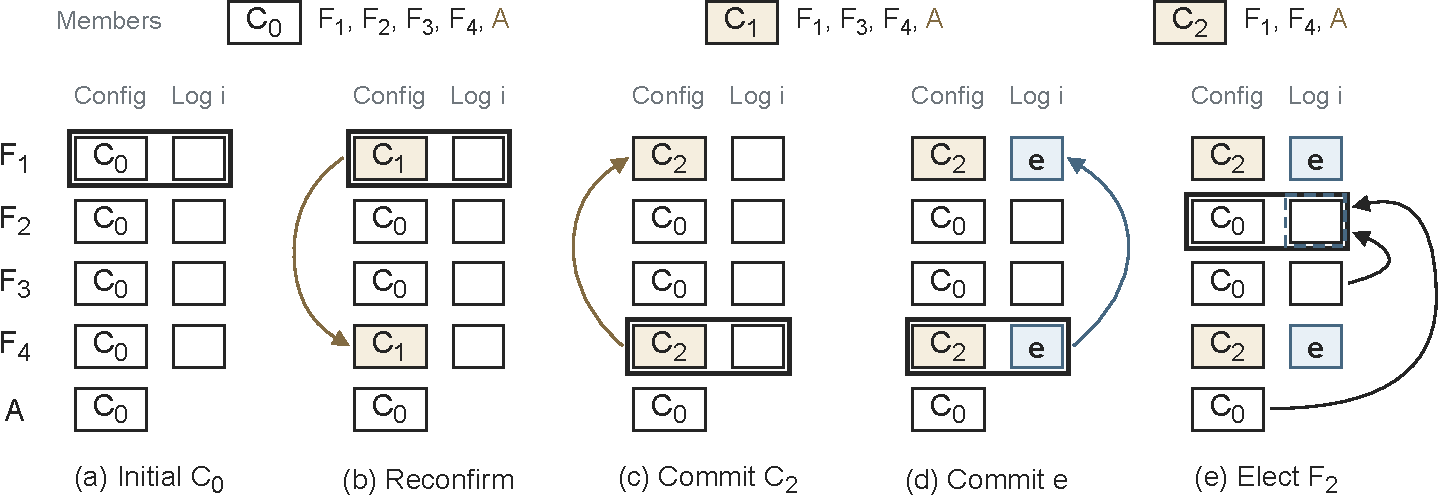
\includegraphics[width=0.64\textwidth]{figures/configuration-confirmation.pdf}
  \caption{Without confirming the inherited configuration, \(F_1\) and
  \(F_4\) commit \(e\) under \(C_2\), yet \(F_2,F_3,A\) still elect
  \(F_2\) under \(C_0\) without \(e\). Had \(F_1,F_3,F_4\) first
  confirmed \(C_1\) in proposal~2, \(F_3\) would have rejected \(F_2\)'s
  Prepare in proposal~3. \emph{Config} shows the installed configuration;
  an empty \emph{Log \(i\)} cell lacks \(e\). Reproduced
  from~\cite[Fig.~4]{arbitration}.}
  \Description{Five snapshots of a four-full-replica stream and arbiter.
  Rows show local configurations and the entry at position i. After two
  successive removals, F1 and F4 hold e while F2, F3, and A retain the
  original configuration and can elect F2.}
  \label{fig:confirmation}
\end{figure*}

After recovery, a proposer must confirm the inherited membership with a
majority of its election voters in its own proposal before proposing any
prefix or changing membership. Each subsequent change requires
confirmation by a majority of the new election membership before the
proposer can use its accept quorum or issue another change. In the
figure, confirming \(C_1\) requires at least one of \(F_3\) and \(A\).
Either voter would then reject the illustrated Prepare under \(C_0\).

% Separate q and u so the small-caps heading copies correctly from the PDF.
\begin{lemma}[Prepare q\kern0pt uorum intersection]\label{lem:prepare}
Fix a proposal number \(q>0\). Let \(C\) be the newest configuration
confirmed in a proposal below \(q\), taking \(C_0\) as confirmed in proposal~0.
\begin{enumerate}
  \item[\emph{(a)}] Any two Prepares that complete at \(q\) have
    intersecting prepare quorums.
  \item[\emph{(b)}] Each such Prepare uses a version at least as recent
    as \(C\), and its prepare quorum intersects every majority that confirmed \(C\).
\end{enumerate}
\end{lemma}

\begin{proof}
We prove Lemmas~\ref{lem:prepare} and~\ref{lem:proposer} jointly by
induction on \(q>0\). By the induction hypothesis, each proposal below
\(q\) has at most one proposer, so configurations issued below \(q\) are
totally ordered by version. Order the configurations confirmed below
\(q\) as \(C_0<C_1<\cdots<C_m=C\). We maintain two invariants for each \(C_k\): (i)~no version older than
\(C_k\) completes Prepare at any higher proposal (\(\le q\)), and
(ii)~versions \(U\) with \(C_k\le U<C_{k+1}\) (or \(U\ge C_m\) issued
before \(q\) for \(k=m\)) use at most two adjacent memberships:
\(P_{C_k}\) and at most one pending one-replica change \(P'\).

For \(C_0\), (i) is vacuous and only \(P_{C_0}\) exists. Between \(C_k\)
and \(C_{k+1}\), \(C_k\)'s proposer publishes at most one unconfirmed
change \(P'\). Any higher proposer before \(C_{k+1}\) prepares with a
version \(\ge C_k\) by~(i), so it inherits \(P_{C_k}\) or \(P'\); since
it must confirm that membership before changing it, any unconfirmed
reconfirmation it issues introduces no third membership. Thus~(ii)
holds, and \(C_{k+1}\) has membership \(P_{C_k}\) or \(P'\), which is
equal or adjacent to both. For any Prepare at proposal \(r\le q\) above
\(C_{k+1}\)'s proposal \(t\) using a version \(U\) with
\(C_k\le U<C_{k+1}\), the confirming majority of \(C_{k+1}\) intersects
\(U\)'s prepare quorum: the shared voter either confirmed \(C_{k+1}\)
first (setting \(\mathit{config}\ge C_{k+1}>U\) and rejecting \(U\)) or
granted Prepare at \(r\) first (setting \(\mathit{promise}\ge r>t\) and
rejecting confirmation at \(t\)). Older versions remain excluded by~(i),
preserving~(i) for \(C_{k+1}\).

Applying~(i) and~(ii) to \(C=C_m\): every Prepare completing at \(q\)
uses a version \(\ge C\) whose membership is \(P_C\) or \(P'\). Since
these memberships are equal or adjacent, their majorities intersect,
giving~(a) and~(b) (the shared voter with a confirming majority of \(C\)
may be \(A\)).
\end{proof}

\subsection{One Proposer per Proposal Number}
\label{sec:proposer}
\begin{lemma}[Proposer uniq\kern0pt ueness]\label{lem:proposer}
For each proposal number \(q>0\), at most one proposer completes Prepare.
\end{lemma}

\begin{proof}
By Lemma~\ref{lem:prepare}(a), any two candidates that obtain
prepare quorums at \(q\) share a voter. Because granting Prepare at
\(q\) requires \(q>\mathit{promise}\) and immediately sets
\(\mathit{promise}:=q\), a common voter cannot grant Prepare at \(q\) to
two candidates. This establishes uniqueness at \(q\) and completes the
joint induction.
\end{proof}

\subsection{Recovery Preserves Committed Entries}
\label{sec:recovery}
\begin{lemma}[Committed-prefix preservation]\label{lem:recovery}
Let \(X\) be the log prefix ending with an entry committed at LSN \(i\)
in proposal \(p\). Upon completing recovery, every full-replica leader
of a proposal \(q>p\) obtains a recovered prefix \(P_{\mathrm{rec}}(q)\)
extending \(X\).
\end{lemma}

\begin{proof}
Fix an entry \(e\) committed at LSN \(i\) in proposal \(p\), and let
\(X\) be the leader's prefix through \(i\). Induct on \(q>p\): assume
every full-replica proposer at \(r\in(p,q)\) recovered a prefix
extending \(X\).

Every transition preserves \(\acc\le\mathit{promise}\). Hence any full
replica in \(q\)'s prepare quorum \(Q_1\) that grants Prepare at \(q\)
had \(\acc\le\mathit{promise}<q\) prior to granting it, so its reply
\((r,j)\)---reporting durable \(r=\acc\) and log end LSN \(j\)---satisfies
\(r<q\). Because \(\mathrm{Accept}\) is the sole transition that updates
durable \((\acc,\mathrm{log})\), two invariants hold on every full
replica:
\emph{(i)~Monotonicity:} \((\acc,\ell)\) is lexicographically
nondecreasing (\(t\ge\mathit{promise}\ge\acc\), and \(t=\acc\) retains
the longer prefix).
\emph{(ii)~Prefix validity:} whenever \(\acc=r>0\), \(r\) belongs to a
full-replica proposer (as \(A\) never proposes redo), and the replica's
log is a prefix of proposal~\(r\)'s sole leader's log extending
\(P_{\mathrm{rec}}(r)\).

It therefore suffices to exhibit one full replica \(F\in Q_1\) supplying
a reply \((r_0,j_0)\ge(p,i)\) in lexicographic order. The selected pair
\((r,j)\) then satisfies \((r,j)\ge(p,i)\) with \(r<q\). By prefix
validity and Lemma~\ref{lem:proposer}, if \(r=p\) then \(j\ge i\) and
the selected prefix is proposal~\(p\)'s log through \(j\), which
contains \(X\) by the append-only rule; if \(p<r<q\), proposer~\(r\)
recovered \(X\) by induction and the selected prefix extends
\(P_{\mathrm{rec}}(r)\), so it again contains \(X\).

\noindent\emph{Configuration lineage.}\enspace
Each configuration \(W\neq C_0\) has a unique parent from which it
arises by reconfirmation (preserving membership) or by a membership
change. Let \(D\) be the configuration in effect when \(p\) committed
\(X\) (confirmed in \(p\)), and \(V\) the configuration used by Prepare
at \(q\). Lemma~\ref{lem:prepare}(b) gives \(V\ge D\). Moreover, every
configuration \(W\ge D\) descends from \(D\) along this parent chain:
within \(p\), Lemma~\ref{lem:proposer} gives one proposer; for any
\(r>p\), Lemma~\ref{lem:prepare}(b) ensures Prepare uses a version
\(\ge D\) below \(r\), which descends from \(D\) by induction.

\emph{Case 1: No membership change occurred after \(D\) on \(V\)'s
lineage.}
Then \(V\) shares \(D\)'s membership (\(S_V=S_D, P_V=P_D\)).
Committing \(X\) under \(D\) required an accept quorum of \(S_D\) to
accept the prefix through \(i\) in proposal \(p\). By
Lemma~\ref{lem:quorum}, that quorum intersects \(Q_1\) in a full replica
\(F\). Because \(F\) rejects \(\mathrm{Accept}(p,\cdot)\) once
\(\mathit{promise}\ge q>p\), it accepted the prefix through \(i\) in
\(p\) before granting Prepare at \(q\), setting \((\acc,\ell)\ge(p,i)\).
By monotonicity, \(F\) replies \((r,j)\ge(p,i)\).

\emph{Case 2: Some membership change occurred after \(D\) on \(V\)'s
lineage.}
Let \(M_1\) and \(M\) be the first and last such changes, and let
\(t_M\) be \(M\)'s issuing proposal and \(b\) the end LSN of \(M\)'s
pre-change synchronized prefix. Since no further change follows \(M\),
\(S_V=S_M\) and \(P_V=P_M\). Because \(D<M\le V\) and \(q\) exceeds
\(V\)'s issuing proposal, we have \(p\le t_M<q\). Moreover, \(b\ge i\): if \(t_M>p\), proposer~\(t_M\) recovered \(X\) by
induction before synchronizing \(M\); if \(t_M=p\), both \(M_1\) and
\(M\) were issued in \(p\) after \(D\), and because \(p\) froze \(D\)'s
commit point no later than when it selected \(M_1\)'s pre-change
synchronization prefix (without canceling \(M_1\) to resume committing
under \(D\)), committing \(X\) at \(i\) under \(D\) preceded selecting
\(M_1\)'s prefix, so append-only gives \(b\ge i\). Before publishing
\(M\) in \(t_M\), pre-change log synchronization had an accept quorum
\(R\subseteq S_M\) accept the prefix through \(b\ge i\) in \(t_M\). By
Lemma~\ref{lem:quorum}, \(R\) intersects \(Q_1\) in a full replica
\(F\). Since \(t_M<q\), \(F\) accepted that prefix in \(t_M\) before
granting Prepare at \(q\), setting \((\acc,\ell)\ge(t_M,b)\ge(p,i)\). By
monotonicity, \(F\) replies \((r,j)\ge(p,i)\), completing the induction.
\end{proof}

\balance
\subsection{Leader Completeness and Agreement}
\label{sec:agreement}
\begin{proof}[Proof of Theorem 4.3]
By Lemma~\ref{lem:recovery}, every higher-numbered full-replica leader's
recovered prefix holds \(e\) at \(i\). Within one proposal,
Lemma~\ref{lem:proposer} gives a single append-only proposer, so two
commits cannot disagree at \(i\). Across proposals, the higher-numbered
leader proposes only prefixes extending its recovered prefix (holding
\(e\) at \(i\)) and only appends, preventing disagreement at \(i\).
\end{proof}

\subsection{Liveness}
\label{sec:liveness}

\textit{Progress assumptions.} The stream starts with \(2k\) healthy
full replicas and one healthy arbiter \(A\) (\(k\ge 1\)). At most
\(k\) members fail and never recover. Among survivors, each emitted
message (request or reply) is eventually delivered once, storage
operations complete, and continuously enabled actions execute. Only
failed full replicas are degraded, no full replicas are added, and each
needed degradation is eventually attempted. Eventually, a surviving full
replica initiates and retains a proposal \(q\) higher than all
previously initiated proposals, with no competing proposer thereafter. At
the start of \(q\), its installed configuration is at least as recent as
every configuration held by a survivor or still deliverable from an
earlier proposal.

\noindent\textsc{Theorem 4.4 (Liveness).}
\emph{Under these progress assumptions, a full replica eventually
completes log reconfirmation and remains leader. Every write it
subsequently accepts eventually commits.}

\begin{proof}
Consider the surviving full-replica candidate \(c\) and proposal \(q\)
guaranteed by the progress assumptions (after the last failure, or from
the initial state if none fails), and let \(W\) be \(c\)'s installed
configuration at the start of \(q\). Every surviving full replica still
belongs to \(W\)'s membership, since only failed replicas are degraded.
Because \(q\) exceeds all previously initiated proposals and no
competing proposer acts thereafter, every surviving voter satisfies
\(\mathit{promise}<q\) when \(\mathrm{Prepare}(q,W)\) arrives; because
\(W\) is at least as recent as every configuration held by a survivor or
still deliverable from an earlier proposal, every surviving voter also
satisfies \(\mathit{config}\le W\). Hence every surviving voter in
\(P_W\) grants \(\mathrm{Prepare}(q,W)\) (setting
\(\mathit{promise}:=q\)), and all subsequent confirmation and
\(\mathrm{Accept}\) requests from \(c\) in \(q\) satisfy
\(q\ge\mathit{promise}\) and version~\(\ge\mathit{config}\) on every
survivor.

\emph{At least \(k+1\) full replicas survive.} Even in \(C_0\)
(\(|S_{C_0}|=2k\), \(|P_{C_0}|=2k+1\)), these survivors form both a
prepare quorum and an accept quorum, and degradations only shrink quorum
sizes. Thus \(c\) completes \(\mathrm{Prepare}(q,W)\), computes
\(P_{\mathrm{rec}}(q)\), confirms \(W\) in \(q\), and has a live
accept quorum accept \(P_{\mathrm{rec}}(q)\) in \(q\) without
degradation.

\emph{Exactly \(k\) full replicas survive.} Since at most \(k\) members
failed, \(A\) is live. Together the \(k\) survivors and \(A\) provide
\(k+1\) voters, forming a prepare quorum of \(P_W\) (size \(\le 2k+1\)),
so \(c\) completes \(\mathrm{Prepare}(q,W)\), computes
\(P_{\mathrm{rec}}(q)\), and confirms \(W\) in \(q\). If \(W\) already removed all \(k\) failed replicas, \(|S_W|=k\) and the
\(k\) survivors directly accept \(P_{\mathrm{rec}}(q)\) in \(q\).
Otherwise, suppose \(m<k\) failed replicas have been removed so far
(\(|S_W|=2k-m\)). Removing one failed replica leaves \(2k-m-1\) full
replicas (accept quorum size
\(\lfloor(2k-m-1)/2\rfloor+1 = k-\lfloor m/2\rfloor \le k\)) and
election membership size \(2k-m\le 2k\) (majority \(\le k+1\)). Thus
the \(k\) survivors complete pre-change log synchronization for
\(P_{\mathrm{rec}}(q)\) in \(q\), the candidate publishes the removal,
and the \(k\) survivors with \(A\) confirm it in \(q\). Each further
degradation completes identically (at most \(k\) failures exist).

Once the effective configuration is confirmed and a live accept quorum
accepts \(P_{\mathrm{rec}}(q)\) in \(q\), the stable leader completes
log reconfirmation (recovery, confirmation, and \(P_{\mathrm{rec}}(q)\)
acceptance) and serves writes; each subsequent write is appended,
accepted by a live accept quorum in \(q\), and committed.
\end{proof}

\begin{thebibliography}{2}
\bibitem{lamport}
Leslie Lamport. 2005.
\newblock \emph{Generalized Consensus and Paxos}.
\newblock Technical Report MSR-TR-2005-33. Microsoft Research.
\newblock \url{https://www.microsoft.com/en-us/research/wp-content/uploads/2016/02/tr-2005-33.pdf}

\bibitem{arbitration}
Quanqing Xu, Chen Qian, Chuanhui Yang, Hao Liu, Wanhong Wang,
Guoping Wang, Fusheng Han, Hanyi Liu, Siyu Mao, Xiu Tang,
Dongxiang Zhang, and Gang Chen.
\newblock \emph{Arbitration Without Redo: Data-less Voting for Site-Level
Disaster Recovery in OceanBase}.
\end{thebibliography}
\end{document}
